\chapter{How to run the ANITA-3 binned analysis}

The \gls{anita} binned analysis software is maintained, backed up and version-controlled on GitHub at the link: 

\begin{center}
\href{https://github.com/osu-particle-astrophysics/BinnedAnalysis}{https://github.com/osu-particle-astrophysics/BinnedAnalysis} 
\end{center}

Inside this repository, there exist code to perform the binned analysis for \gls{anita}-2 as well as code for \gls{anita}-3. 
These are located in the directories called \path{anita2code} and \path{anita3code}, respectively. 
In this appendix, we will cover how to run the analysis for \gls{anita}-3. Note that the \gls{anita}-3 analysis could be adapted to work for \gls{anita}-4. The \gls{anita}-2 flight had a significantly different triggering system, among other differences, making it difficult to adapt its analysis to newer flights. However, I will try to include a separate note on how to run the binned analysis for \gls{anita}-2 as well. 

Doing the \gls{anita}-3 binned analysis involves running a set of code. Details on the development of this code base can be found in~\cite{brianDaileyThesis,samStaffordThesis,jacobGordonThesis} and in various chapters of this thesis. 
To run the analysis, the order of operations to follow are below. 

\begin{center}
Run interferometry\\
Run analysis stage 1\\
Run analysis stage 2\\
Optimize LD cut\\
Run analysis stage 2 

\end{center}

\section{How to run the interferometry}

Go into the file called runInterferometry.cxx and change two things: the input and the output. Specifically, this might involve setting the variables called \path{dataDirLocal}, \path{outputFilename}, and \path{outputDirStr}. I show below what I have set these to for my current work. 

\begin{center}
dataDirLocal: \path{$OINDREE_SIM/kotera_march30/Energy_222}
\end{center}

This is the simulated data over which I currently want to run the interferometry. It may not be what you need.

What you change this to depends on which simulation data you want to run interferometry over. 

\begin{center}
outputFilename: \path{/fs/scratch/PAS0174/anita/oindree/InterferometryOutput/simKoteraMarch30/geomFilter/analyzerResults..root}
\end{center}

\begin{center}
outputDirStr: \path{$OINDREE}
\end{center}

You should change the outputDirStr and OutputFilename to something else, such as some directory where you want the output.
Then run: 

\begin{center}
make \path{runInterferometry}\\
qsub \path{runInterferometrySim.job}\\
showq -u osu0426 
\end{center}


The last command is to see whether the job started or not. 
A \path{.o} file will appear when the job has finished, check it and make sure everything looks right . Mainly you are checking that the input and output that you intended for it to use is actually being used. Once the job has finished go to the output dir and check the root file \path{analyzerResults*.root} that was made to make sure it looks fine. 
There should be only one root file, for one run. 

We have not run the interferometry for all the runs yet. 
If this looks good we can run interferometry for all the runs now.  This is done by running the following: 
\begin{center}
\path{./runInterferometrySim.sh} 
\end{center}

This starts a job for each run. 

Recap of code files we used for interferometry:  

\begin{center}
\path{runInterferometry.cxx}\\
\path{runInterferometrySim.job}\\
\path{runInterferometrySim.sh}
\end{center}

Also commonly useful to know is how to run the interferometry for a particular event from the real data:

\begin{center}
\path{./runInterferometry -PB --FILTER_OPTION=4,
-BbaselineSampleSmooth_1_2.00.root} 383 69969708
\end{center}

This command will run the interferometry for a single event  69969708 from run 383. 

\begin{itemize}

\item $FILTER\char`_OPTION=4$ invokes the geometric filter with a noise baseline from the file indicated in the -B parameter

\item $FILTER\char`_OPTION=2$ and $SINE\char`_SUBTRACT\char`_THRESHOLD=0.1$ will give a reasonable implemetation of sine subtraction filter

\item $FILTER\char`_OPTION=0$ means no filtering

\item -O parameter directs the output to the directory name contiguously following the -O

\item -G displays the the interferometric maps interactively

\end{itemize}


\section{How to run analysis stage 1}

To run the analysis stage 1, you can compile the associated code as follows:

\begin{center}
make \path{runAnalysisStage01} 
\end{center}

Currently, there are lots of warnings that you get at this stage and that is the ``normal." Next run it as follows. 

For simulation:
\begin{center}
qsub \path{stage01_sim.job}
\end{center}

For data:
\begin{center}
qsub \path{stage01.job}
\end{center}

When stage 1 finishes running, it makes several files in the output folder you assigned.

Most importantly, this file is made as an output from stage 1 : 

\begin{center}
\path{analysisOutput_1_99.root} 
\end{center}

This is from me running the code for simulation with runs going from 1 to 99. 
The run numbers will depend on which runs you had the code run over.
The more runs you run it over the longer it takes.
This file is the input in stage 2 of the analysis, so in that sense this is the most important file because without this you can’t do the next stage of the analysis.

If you want to 
run stage 1 for ONE event from data (ANITA-3), say, for an interesting event such as the mystery event 2 or ME2, this is how you could do it: 

\begin{center}
\path{./runAnalysisStage01} \path{-CA} \path{-9} \path{-D/fs/scratch/PAS0174/anita/2015_05_19/sample_90/geomFilter} 175 439 15717147
\end{center}

This would actually take a while as you are saying to run over all the runs used in the analysis so you would need to run a job with this command (see \path{stage01.job}) 

To save time you could also just run using the run that the particular event is in, e.g. ME2 is in run 176 so you could do : 

\begin{center}
\path{./runAnalysisStage01} \path{-CA} \path{-9} \path{-D/fs/scratch/PAS0174/anita/2015_05_19/sample_90/geomFilter} 176 176 15717147
\end{center}

The \path{-CA} flag tells the stage 1 code to apply analysis cuts. The \path{-9} flag tells it to use the 90\% data sample. The \path{-D} flag tells it the location of the interferometry results. The 176 and 176 tells it the run(s) to run the code over and the 15717147 is the specific event number for which the code would be run. When an event number is not specified at the end then the code is run for all events in the specified runs. 

When you get to the point of running stage 1 and have made the \path{analysisOutput....root} file, you should try looking inside that file and see what things are in there and try to visualize them to get a better idea. 


\section{How to run analysis stage 2}

The stage 2 code is run twice, once before the optimize code and once after. In this section, we discuss how to run it before the optimize code. 

The stage 2 code takes as input a file that was output from the stage 1 code:

\begin{center}
\path{analysisOutput_188_193.root} 
\end{center}

The above file is made by running the stage 1 code over the \gls{anita}-3 data using runs 188 through 193. If other runs were used the associated run numbers would appear in the filename instead. If stage 2 also needs to be run over those same runs then the following command can be used:

\begin{center}
\path{./runAnalysisStage02} \path{-D/fs/scratch/PAS0174/anita/oindree/Stage1Output/BgOnly/GRB1} \path{-I/fs/scratch/PAS0174/anita/2015_05_19/sample_10/geomFilter} 188 193 \path{-b} \path{-PV} \path{-S_v} \path{-FanalysisOutput_188_193.root}
\end{center}

The -D flag tells the stage 2 code where the file output from stage 1 is. The -I flag tells the code where the associated results from running the interferometry is. 188 and 193 are the start and end runs over which stage 2 will run. -b tells it to re-bin. -PV tells it to run for \gls{vpol}. \path{-S_v} labels an output file with the subscript \path{_v} denoting \gls{vpol}. The -F flag tells the stage 2 code the name of the input file from stage 1 that it has to use.

When stage 2 finishes running it also makes a file called \path{analysisOutput_188_193.root}, for example, which can then be used as input by the optimize code. 

\section{How to run the optimize code}

Before running the optimize code, make sure to change the variables \path{outputDir} and \path{inFilename}. To run the optimize code using the optimized healpix orientations, use the following commands. 

\begin{center}
\gls{vpol}:
\path{./optimizeLDCut} \path{-pV} \path{-r} \path{--PHI_HP_OFFSET=.56} \path{--THETA_HP_OFFSET=-5.04}
\end{center}

\begin{center}
\gls{hpol}:
\path{./optimizeLDCut} \path{-pH} \path{-r} \path{--PHI_HP_OFFSET=3.92} \path{--THETA_HP_OFFSET=0.00}
\end{center}


\section{How to run analysis stage 2 again}

After optimizing, the stage 2 analysis must be run again - this time, with final cuts. This should be the last step of the analysis resulting in finding out which events pass all cuts. To run the stage 2 analysis with final cuts for \gls{vpol} run something like this command: 

\begin{center}
\path{./runAnalysisStage02} \path{-b} \path{-D/users/PAS0654/osu0426/BinnedAnalysis/anita3code/Diffuse/stage2inputs/fullDataSet} \path{-I/fs/scratch/PAS0174/anita/2015_05_19/sample_90/geomFilter} 175 439 \path{-PV} \path{-S_v} \path{-a} \path{-FanalysisOutput_175_439.root}
\end{center}

The \path{-a} says to apply final cuts.  
Use it when optimizeLDCut has been run and you want to know which events pass all cuts. Things are getting serious now!

In order to successfully run stage 2 with final cuts, you need two files per polarization. First, you need to provide a file containing the bin numbers of bins that you will be using for your search. These should be named as follows. 

\begin{center}
\path{binsOver0.01_h.txt}\\
\path{binsOver0.01_v.txt}
\end{center}

You will know the final bins to use for the search from the table produced in the optimize step called something like \path{oindree_optimization_final_sl_06_sf_0.020654.txt}. This table also needs to be provided to stage 2 as an input. Re-name the \path{oindree_optimization_final_sl_06_sf_0.020654.txt} file as the following before doing so. 

\begin{center}
\path{intercept_h.txt}\\
\path{intercept_v.txt}
\end{center}

A screenshot of an example table is shown in Figure~\ref{opt_table}. Note that the eighth column from the left shows the optimized LD cut for each bin. This information, for example, is needed to run stage 2 with final cuts. 

\begin{figure}
\centering
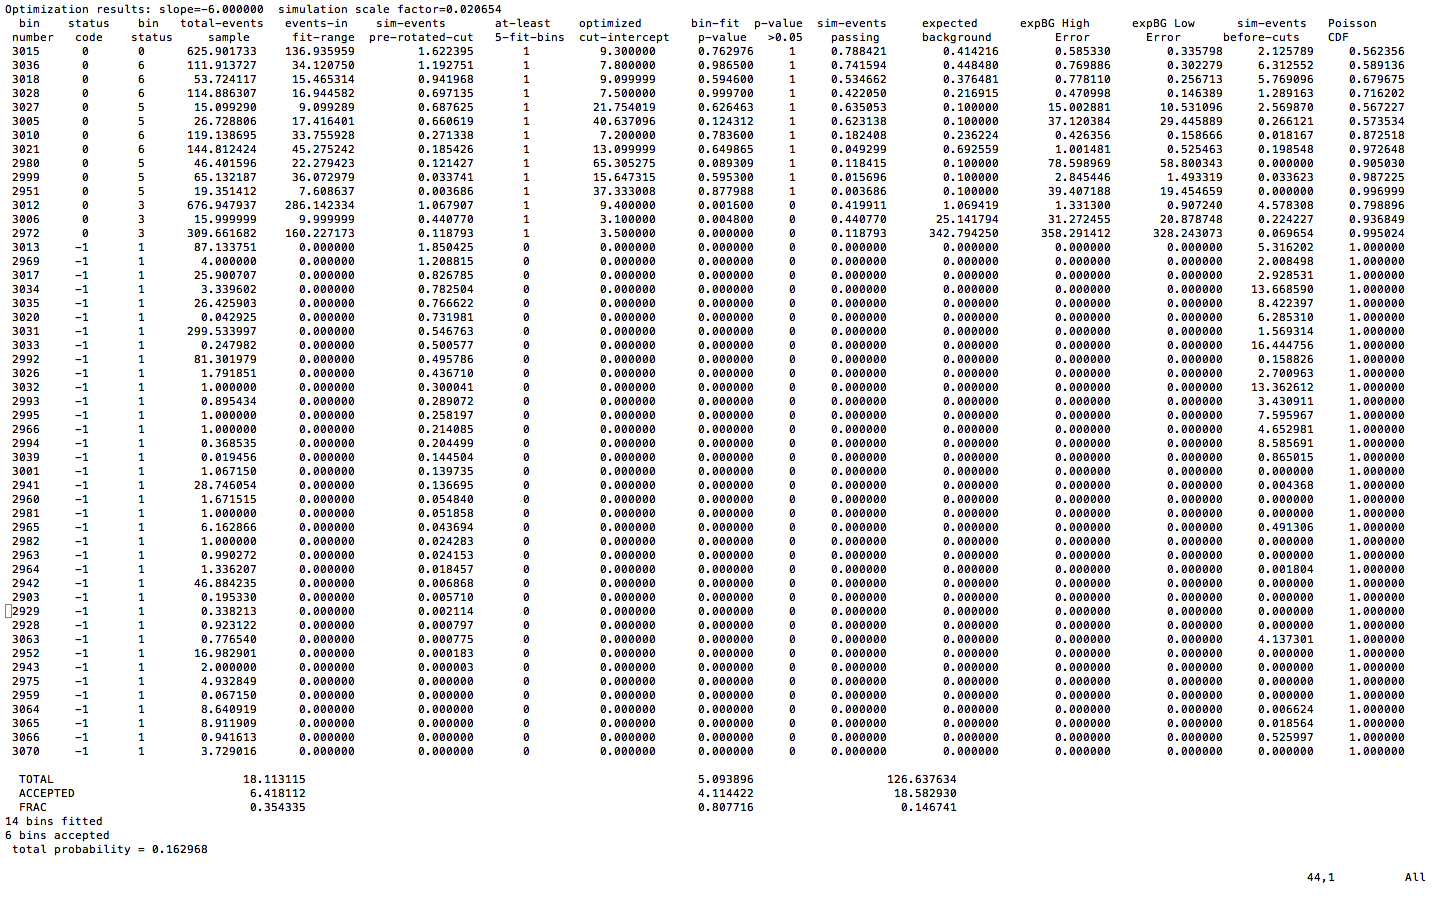
\includegraphics[width=1.0\textwidth]{figures/optimize_table.png}
\caption{The table produced by the optimize code and needs to be used as input to run the stage 2 analysis with final cuts.}
\label{opt_table}
\end{figure}














